% Full chain: pdflatex -> bibtex -> pdflatex -> pdflatex
\documentclass[11pt,en,cite=authoryear]{elegantpaper}

\title{Circulation theory of enzyme kinetics}

\author{Yuhao Jiang}
\date{\today}

%command
\usepackage{array}
\usepackage{amssymb}
\usepackage{graphicx,float,subfigure}
\usepackage{subfigure}
\usepackage[T1]{fontenc}
\usepackage[utf8]{inputenc}
\usepackage{mathtools}
\usepackage{bm}

\begin{document}

\maketitle
We consider the following m-step($n\ge 2$) enzyme kinetics model:
\begin{align} \label{eq:model}
    \bm{E + S \rightleftharpoons
    ES \rightleftharpoons
    EP_1 \rightleftharpoons
    EP_2 \rightleftharpoons
    \cdots
    EP_{m-2} \rightleftharpoons
    E + P}
\end{align}

where $\bm{E}$ is an enzyme turning the substrate $\bm{S}$ into the product $\bm{P}$. From the  perspective of a single enzyme molecule, this enzyme kinetics can be modeled as n-step Markov chain $(\xi_l)_{l\ge 0}$, with finite state space S defined on some space $(\Omega, \mathcal{F}, P)$. When $n=2$, this Markov chain only have two state $\bm{E}$ and $\bm{ES}$, we say that the state space $S=\{1, 2\}$.

\begin{definition}
    Let $\mathbb{Z}$ be the set of integers, and a periodic function $f$ which maps $\mathbb{Z}$ to S is called circuit function. If $s$ is the smallest positive integer which satisfied $f(n+s) = f(n)$ for $\forall n \in \mathbb{Z}$, then we called it the period of $f$.
\end{definition}

\begin{definition}
    Two circuit functions $f$ and $g$ in S are called equivalent if there exists some $m \in \mathbb{Z}$ such that $g(n) = f(n+m)$ for $\forall n \in \mathbb{Z}$.
\end{definition}
\begin{definition}
    For a circuit function $f$ in S with period $s$ that satisfies $f(1)=i_1$, $f(2)=i_2$, $f(3)=i_3$. The equivalence class that $f$ belongs is a cycle $c=(i_1, i_2, \dots i_s)$
\end{definition}

According to above definitions, $c_1 = (1, 2, 3), c_2 = (3, 1, 2)$ and $c_3 = (2, 3, 1)$ represent the same cycle. So a cycle is also a equivalence class on the space of all circuit functions under the equivalence relation.

For presentation purposes, if the order sequence $i_1, i_2, \dots, i_s$ occurs in the cycle $c$ continuously, we denote that $[i_1, i_2, \dots, i_s] \in c$. Specially, if $[i_1] \in c$, the point $i_1$ occurrs in $c$, and $[i_1, i_2] \in c$ denotes the edge $i_1 i_2$ exists in the cycle $c$. 
For the cycle $c_1 = (1,2)$, we use $k_{12}$ to denote the number of cycle $c_1$.

\begin{definition}
    Let $\mathcal{C}_n(\omega)$ be the class of cycles occurring along the sample path $(\xi_l)_{l\ge 0}$ until time $n$. Then we use $\mathcal{C}_{\infty}$ to represent the limit of $\mathcal{C}_n$ as $n \rightarrow \infty$. This convergence has been proofed in [].
\end{definition}

\begin{definition} %% follow Jia2016
    Let $k_{c, n}$ denote the number of time that cycle c is formed by a Markov chain up to time $n$. Then the sample circulation $J_{n}^c$ along cycle $c$ by time $t$ is defined as
    $$
    J_{n}^c = \frac{1}{n} k_{c, n} \quad \forall c \in \mathcal{C}_{\infty}
    $$
    and the circulation $w^c$ along cycle $c$ is a nonnegative real number defined as the following almost sure limit:
    $$
    w_c = \lim_{n \rightarrow \infty} J_{n}^c \quad \forall c \in \mathcal{C}_{\infty}, \quad a.s.
    $$
    which represents the number of times that cycle $c$ ic formed per unit time. Let $J_n = (J_n^c)_{c \in C_{\infty}}$ and $w =  (w_c)_{c \in C_{\infty}}$.
\end{definition}

For the enzyme kinetics model, if the state space $S=\{1, 2, \dots, m\}$, then $\mathcal{C}_{\infty}$ has $2m+2$ cycles, including $n$ 1-state cycles, $n$ two-state cycles and two n-state cycles

Let $|c|$ denotes the length of cycle $c$, and 
$E = \{\mu=(\mu_c)_{c\in \mathcal{C}_{\infty}} \in [0, 1]^r :\sum_{c \in \mathcal{C}_{\infty}} |c| \mu_c  = 1\}$, then the circulation distribution $w = (w_{c})_{c \in \mathcal{C}_{\infty}} \in E$.

\begin{definition}
    We say that $J_{n}^c$ satisfies a large deviation principle with rate $n$ and good rate function $I$ : $E \rightarrow [0, \infty]$ if:
    \begin{align}
        \lim_{n \rightarrow \infty} \frac{1}{n} \log \mathbb{P}(J_{n}^c = \nu_c , c \in \mathcal{C}_{\infty}) = - I(\nu), \quad \forall \nu
    \end{align}
    where $\sum_{c \in \mathcal{C}_{\infty}} |c| \nu_c = 1$, 
    % $r$ is the size of set $\mathcal{C}_{\infty}$,
    and $\nu = (\nu_c)_{c \in \mathcal{C}_{\infty}} \in E$.
\end{definition}


\section{Large deviation of circulation for finite Markov chains}

\subsection{Large deviation of circulation for three state Markov chains}

\begin{theorem}
    \begin{figure}[h]
        \centering
        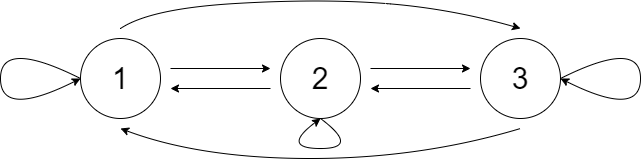
\includegraphics[scale=0.3]{3-state.png}
        \caption{3-state transition diagram}
    \end{figure}

For the three-state Markov chains, let $S = \{1, 2, 3\}$, $J_{n}$ satisfies a large deviation principle, and its rate function is
\begin{align}
    I_3^c(\nu) &= \sum_{c \in \mathcal{C}_{\infty}} \nu_{c} \log \frac{\nu_{c}}{w_c} + \sum_{i\in S}(\nu^i - \nu_i)\log \frac{\nu^i - \nu_i}{w^i - w_i} \\
    &-(\tilde{\nu} - \sum_{i\in S}\nu_i)\log(\frac{\tilde{\nu} - \sum_{i\in S}\nu_i}{\tilde{w} - \sum_{i\in I}w_i}) \\
    &-\sum_{i\in S} \nu^i \log (\frac{\nu^i}{w^i})
\end{align}
where $S=\{1, 2, 3\}$ is the state space for Markov chains。
$$\mathcal{C}_{\infty}^3 = \{(1), (2), (3), (1,2), (2,3), (1,3), (1,2,3), (1,3,2)\}$$
is the class of all cycles occurring.
$\nu_c$ is the frequence of cycle $c$ occurring, $w_c$ is the cycle skipping rate on $c$.\\
Let $\nu^{i} = \sum_{c \supseteq (i)} \nu_{c}$, such as $\nu^{1} = \nu_{1} + \nu_{12} + \nu_{13} + \nu_{123} +\nu_{132}$.
Let  $\tilde{\nu} = \nu_{1} + \nu_{2} + \nu_{3} + \nu_{12} + \nu_{13} + \nu_{23} + \nu_{123} +\nu_{132}$ represent the sum of all the elements of $\nu$. 
And $w^i$, $w_i$ is similarly defined for $w$.
\end{theorem}
\begin{proof}
    For the n-step path, after counting all the cycles, it maybe remain some points which haven't form cycles, we call this chain the derived chains.
    Refer to the Appendix, $\mathcal{E} (G^3(k))$ represents the amount of path with $k$ cycle occuring, and $\Pi_{i,j \in S} p_{ij}^{\sum_{c \ni [i,j]} k_{c}} $ is the probability of the part formed all cycles. Obviously, the length of the derived chains is no more than 2 (the amount of states is three), then
    $\min_{\{i, j\}} p_{ij}^{2}$, $\max_{\{i, j\}} p_{ij}^2$ are the lower and upper bound respectively. So
    \begin{align*}
        \mathbb{P}(J_{n}^c= \frac{k_c}{n}, c \in \mathcal{C}_{\infty}) 
        \ge \mathcal{E} (G^3(k)) \Pi_{i,j \in S} p_{ij}^{\sum_{c \ni [i,j]} k_{c}}
        \min_{\{i, j\}} p_{ij}^{2}
    \end{align*}
    The length of the derived chains is no more than 2. And the steps in the derived chains is included in the n steps, so
    \begin{align*}
        \mathbb{P}(J_{n}^c = \frac{k_c}{n}, c \in \mathcal{C}_{\infty}) 
        \le \binom{n}{2}
        \mathcal{E} (G^3(k)) \Pi_{i,j \in S} p_{ij}^{\sum_{c \ni [i,j]} k_{c}}
        \max_{\{i, j\}} p_{ij}^2
    \end{align*}

    We know
    \begin{align*}
        \frac{1}{n} \log \binom{n}{2} \le \frac{1}{n} \log \frac{n^2}{(2)^{2}}
        = O(\frac{\log n}{n})
    \end{align*}
    so 
    \begin{align*}
        \mathbb{P}(J_{n}^c = \frac{k_c}{n}, c \in \mathcal{C}_{\infty}) 
        = \exp(O (\log n))
        \mathcal{E} (G(k)) \Pi_{i,j \in S} p_{ij}^{\sum_{c \ni [i,j]} k_{c}}
    \end{align*}
    We could neglect the influence of the derived chains.

    Let
    \begin{align*}
        K_n = \biggl\{k=(k_c)_{c\in \mathcal{C}_{\infty}}: \sum_{c \in \mathcal{C}_{\infty}} k_{c} |c| \le n \biggr\},
    \end{align*}
    and this set includes all possible situations of each cycles occuring amount. It can easily observe that the size of this set $|K_n| \le n^3$, $\frac{1}{n} K_n \in E$. 

    For $\forall k \in K_n$, let $\mu_n(k) = \frac{1}{n} k \in E$. Let us put
    \begin{align*}
        Q_n(a) = \max_{k\in K_n: \mu_n(k) \in B_a(\nu)} 
        \mathcal{E} (G(k)) \Pi_{i,j \in S} p_{ij}^{\sum_{c \ni [i,j]} k_{c}}
    \end{align*}
    where $B_a(\nu)$ is the open neighborhood of $\nu$ with the total vaiation distance
    $ d(\alpha, \beta) = \frac{1}{2} \sum_{s=1}^r |\alpha_s - \beta_s| $ and radius $a$. 
    For enough large n, clearly
    \begin{align*}
        Q_n(a) 
        \le \mathbb{P}(J_{n} \in B_a(\nu), c \in \mathcal{C}_{\infty})
        \le |K_n| Q_n(a).
    \end{align*}

    Stirling's formula gives
    $\frac{1}{n} \log \binom{k}{k'} = h(\frac{k}{n} ) - h(\frac{k'}{n}) - h(\frac{k-k'}{n}) + O(\frac{\log n}{n})$
    where $h(x)=x\log(x)$. We find that

    \begin{align*}
        &\frac{1}{n} \log \mathcal{E} (G^3(k)) \Pi_{i, j \in S} p_{ij}^{\sum_{c \ni [i,j]} k_{c}} \\
        &= h(\nu_{12} + \nu_{13} + \nu_{23}+\nu_{123}+\nu_{132}) 
        + h(\nu_1 + \nu_{12} + \nu_{13} + \nu_{123} +\nu_{132}) \\
        &+ h(\nu_2 + \nu_{12} + \nu_{123} + \nu_{132} +\nu_{23})
        + h(\nu_3 + \nu_{13} +\nu_{123} +\nu_{132} +\nu_{23}) \\
        &- \left[h(\nu_1) + h(\nu_2) + h(\nu_3) + h(\nu_{12}) + h(\nu_{13}) + h(\nu_{23}) + h(\nu_{123}) + h(\nu_{132})\right] \\
        &- \biggl(h(\nu_{12} + \nu_{13} + \nu_{123} +\nu_{132}) + h(\nu_{12} + \nu_{123} + \nu_{132} +\nu_{23}) \\
        & + h(\nu_{13} +\nu_{123} +\nu_{132} +\nu_{23})\biggr)
        +\sum_{i, j \in S, p_{ij}\neq 0} (\sum_{c \ni[i, j]} \nu_{c}) \log p_{ij} + O(\frac{\log n}{n})
    \end{align*}

    Merging all the same items, then
    \begin{align*}
        &\frac{1}{n} \log \mathcal{E} (G^3(k)) \Pi_{i, j \in S} p_{ij}^{\sum_{c \ni [i,j]} k_{c}} \\
        &= -\biggl(
        \nu_1 \log(\frac{1}{p_{1}} \frac{\nu_1}{\nu^1})
        + \nu_2 \log(\frac{1}{p_{2}} \frac{\nu_2}{\nu^2})
        + \nu_3 \log(\frac{1}{p_{3}} \frac{\nu_3}{\nu^3}) \\
        &+\nu_{12} \log(\frac{1}{p_{12}p_{21}} \frac{\nu_{12}}{\nu_{12}+\nu_{23}+\nu_{13}+\nu_{123}+\nu_{132}} 
        \frac{\nu^{1}-\nu_{1}}{\nu^{1}}\frac{\nu^{2}-\nu_{2}}{\nu^{2}}) \\
        &+ \nu_{13} \log(\frac{1}{p_{13}p_{31}} \frac{\nu_{13}}{\nu_{12}+\nu_{23}+\nu_{13}+\nu_{123}+\nu_{132}}
        \frac{\nu^{1}-\nu_{1}}{\nu^{1}}\frac{\nu^{3}-\nu_{3}}{\nu^{3}}) \\
        &+ \nu_{23} \log(\frac{1}{p_{23}p_{32}} \frac{\nu_{23}}{\nu_{12}+\nu_{23}+\nu_{13}+\nu_{123}+\nu_{132}} 
        \frac{\nu^{3}-\nu_{3}}{\nu^{3}}\frac{\nu^{2}-\nu_{2}}{\nu^{2}}) \\
        &+ \nu_{123} \log(\frac{1}{p_{12}p_{23}p_{31}} \frac{\nu_{123}}{\nu_{12}+\nu_{23}+\nu_{13}+\nu_{123}+\nu_{132}}
        \frac{\nu^{1}-\nu_{1}}{\nu^{1}}\frac{\nu^{2}-\nu_{2}}{\nu^{2}} \frac{\nu^{3}-\nu_{3}}{\nu^{3}}) \\
        &+ \nu_{132} \log(\frac{1}{p_{13}p_{32}p_{21}} \frac{\nu_{132}}{\nu_{12}+\nu_{23}+\nu_{13}+\nu_{123}+\nu_{132}}
        \frac{\nu^{1}-\nu_{1}}{\nu^{1}}\frac{\nu^{2}-\nu_{2}}{\nu^{2}} \frac{\nu^{3}-\nu_{3}}{\nu^{3}}) \biggr)\\
    \end{align*}

    % \begin{align*}
    %     w_{12} &= p_{12}p_{21} \frac{D(\{1, 2\}^c)}{\sum_{i\in I} D(\{i\}^c)} \\
    %     w_{13} &= p_{13}p_{31} \frac{D(\{1, 3\}^c)}{\sum_{i\in I} D(\{i\}^c)} \\
    %     w_{23} &= p_{23}p_{32} \frac{D(\{2, 3\}^c)}{\sum_{i\in I} D(\{i\}^c)} \\
    %     w_{123} &= p_{12}p_{23}p_{31} \frac{D(\{1, 2, 3\}^c)}{\sum_{i\in I} D(\{i\}^c)} \\
    %     w_{132} &= p_{13}p_{32}p_{21} \frac{D(\{1, 2, 3\}^c)}{\sum_{i\in I} D(\{i\}^c)}
    % \end{align*}
    Refer to [Jiang], the calculation formula
    for circulation is:
    \begin{align*}
        w_c = p_{i_1 i_2} p_{i_2 i_3} \cdots p_{i_{m-1} i_1} \frac{D(\{i_1, i_2, \cdots i_s\}^c)}{\sum_{j\in S} D(\{j\}^c)}
    \end{align*}
    With this formula, we know
    \begin{align*}
        w_{12}+w_{13}+w_{23}+w_{123}+w_{132} &= \frac{(1-p_{11})(1-p_{22})(1-p_{33})}{\sum_{i\in I} D(\{i\}^c)} \\
        &= \frac{\Pi_{i, j} D(\{i, j\}^c)}{\sum_{i\in I} D(\{i\}^c)}
    \end{align*}
    Since the property of circulation, $p_{ij} = \frac{\sum_{c \ni [i,j]} w_c}{\sum_{c \ni (i)} w_c}$, So
    \begin{align*}
        &\frac{1}{n} \log \mathcal{E} (G^3(k)) \Pi_{i, j} p_{ij}^{\sum_{c \ni [i,j]} k_{c}} \\
        &= \sum_{c \in \mathcal{C}_{\infty}} \nu_{c} \log \frac{\nu_{c}}{w_c} + \sum_{i\in S}(\nu^i - \nu_i)\log \frac{\nu^i - \nu_i}{w^i - w_i} \\
        &-(\tilde{\nu} - \sum_{i\in S}\nu_i)\log(\frac{\tilde{\nu} - \sum_{i\in S}\nu_i}{\tilde{w} - \sum_{i\in S}w_i}) \\
        &-\sum_{i\in S} \nu^i \log (\frac{\nu^i}{w^i})
    \end{align*}
    Now we find that
    \begin{align*}
        \frac{1}{n} \mathbb{P}(J_n \in B_a(\nu))
        &= O(\frac{\log n}{n}) + \frac{1}{n} \log Q_n(a) \\
        &= O(\frac{\log n}{n}) - \min_{k \in K_n: \mu_n(k) \in B_a(\nu)} I_3^c(\mu_n(k))
    \end{align*}
    And we know:
    (i) $\bigcup_{n\in \mathbb{N}} \{\mu_n(k): k \in K_n\} \bigcap E$ is dense in $E$.
    (ii) $\mu \rightarrow I_3^c(\mu)$ is continuous on $E$.
    It is analogous to the proof of Sanov's Theorem, then
    \begin{align*}
        \lim_{n \rightarrow \infty} \frac{1}{n} \mathbb{P}(J_n \in B_a(\nu)) 
        = -\inf_{k \in K_n: \mu_n(k) \in B_a(\nu)} I_3^c(\nu)
    \end{align*}
    If the size of neighborhood $B_a(\nu)$ is enough small, 
    \begin{align*}
        \lim_{n \rightarrow \infty} \frac{1}{n} \mathbb{P}(J_n = \nu) 
        = - I_3^c(\nu)
    \end{align*}
\end{proof}

\begin{corollary}
    For the two-state Markov chains, we have:
    \begin{align*}
    I_2^c(\nu) &= \nu_{1}\log(\frac{\nu_{1}}{\nu_{1}+\nu_{12}}/\frac{w_{1}}{w_{1}+w_{12}}) + \nu_{2}\log(\frac{w_{2}}{w_{1}+w_{12}}) + 2\nu_{12} \log (\frac{\nu_{12}}{\nu_{1}+\nu_{12}}/\frac{w_{12}}{w_{1}+w_{12}})
\end{align*}
\end{corollary}

\begin{corollary}
    $I_3^c$ is  finite, continuous, positive and strictly convex
\end{corollary}
\begin{proof}
    Since $h(x) = x \log x$ is finite on the interval $[0, 1]$, obviously, $I^c_3(\nu)$ is finite on $E$.
    Spliting item $\sum_{c \in \mathcal{C}_{\infty}} \nu_{c} \log \frac{\nu_{c}}{w_c}$, and employ Log sum inequality.
    \begin{align*}
        I^c_3(\nu) 
        &= \left(\sum_{i\in S} \nu_{i}\log \frac{\nu_{i}}{w_i} + \sum_{i\in S}(\nu^i - \nu_i)\log \frac{\nu^i - \nu_i}{w^i - w_i} 
        - \sum_{i\in S} \nu^i \log \frac{\nu^i}{w^i} \right)\\
        &+ \left(\sum_{c \in \mathcal{C}_{\infty}, c\neq (i)} \nu_{c} \log \frac{\nu_{c}}{w_c} 
        -(\tilde{\nu} - \sum_{i\in S}\nu_i)\log(\frac{\tilde{\nu} - \sum_{i\in S}\nu_i}{\tilde{w} - \sum_{i\in S}w_i}) \right)\\
        &= \sum_{i\in S} \left(\nu_{i}\log \frac{\nu_{i}}{w_i} 
        + (\nu^i - \nu_i)\log \frac{\nu^i - \nu_i}{w^i - w_i} \right)
        - \sum_{i\in S} \nu^i \log \frac{\nu^i}{w^i} \\
        &+ \left(\sum_{c \in \mathcal{C}_{\infty}, c\neq (i)} \nu_{c} \log \frac{\nu_{c}}{w_c} 
        -(\tilde{\nu} - \sum_{i\in S}\nu_i)\log(\frac{\tilde{\nu} - \sum_{i\in S}\nu_i}{\tilde{w} - \sum_{i\in S}w_i}) \right)\\ 
        &= \left(\sum_{i\in S} \nu^i \log \frac{\nu^i}{w^i} 
        - \sum_{i\in S} \nu^i \log \frac{\nu^i}{w^i} \right)\\
        &+ \left( (\tilde{\nu} - \sum_{i\in S}\nu_i)\log(\frac{\tilde{\nu} - \sum_{i\in S}\nu_i}{\tilde{w} - \sum_{i\in S}w_i}) 
        -(\tilde{\nu} - \sum_{i\in S}\nu_i)\log(\frac{\tilde{\nu} - \sum_{i\in S}\nu_i}{\tilde{w} - \sum_{i\in S}w_i}) \right)\\
        &\ge 0
    \end{align*}
    The convex can be proofed with the same way by Log sum inequality.
\end{proof}

\subsection{Large deviation of circulation for  finite state Markov chains}
\begin{theorem}
    For the m-state Markov chains, if the rate function exists, it is
    \begin{align*}
        I_m^c(\nu)
        &= [h(\nu_{12}+\nu_{1 m}+\nu^+ +\nu^-) - h(\nu_{12}) - h(\nu_{1m})+
        h(\nu^+) + h(\nu^-)]
        + \sum_{i \in S} [h(\nu^i) - h(\nu^i-\nu_i)]\\
        &+ \max_{\nu^+_{ij} + \nu^-_{ij} = \nu_{ij}, i\neq 1, j\neq m} \biggl\{
        [h(\nu_{12}+\nu^+_{23}+\nu^+) - h(\nu^+_{23}) - h(\nu_{12}+\nu^+)]\\
        &+[h(\nu^+_{34}+\nu^+_{23}+\nu^+) - h(\mu^+_{34}) - h(\nu^+_{23}+\nu^)]+
        \dots +\\
        &+[h(\nu^+_{m-1,m} + \nu^+_{m-2,m-1} + \nu^+) - h((\nu^+_{m-1,m})- h(\nu^+_{m-2,m-1} + \nu^+)] \\
        &+ [h(\nu_{1m}+ \nu^{-}_{m-1,m}+ \nu^-) -h(\nu^-_{m-1,m}) -h(\nu_{1m}+\nu^-)]\\
        &+ [h(\nu^-_{m-1,m} +\nu^-_{m-2,m-1} +\nu^-) -h(\nu^-_{m-2,m-1}) -h(\nu^-_{m-1,m} +\nu^-)]\\
        &+ \dots +
        + h(\nu^-_{23}+\nu^-_{34}+\nu^-) - h(\nu^-_{23} -h(\nu^-_{34}+\nu^-))\biggr\}
        + \sum_{i,j} (\sum_{c \ni [i,j]}\nu_c) \log p_{ij}
    \end{align*}
\end{theorem}
\begin{proof}
    If the rate function exists, we know:
    \begin{align*}
        I_m^c(\nu) = \frac{1}{n} \log \mathcal{E} (G^m(k)) \Pi_{i, j \in S} p_{ij}^{\sum_{c \ni [i,j]} k_{c}}.
    \end{align*}
    The accumulation part in $\mathcal{E} (G^m(k))$ has no more than $n^{m-1}$ items, and $\frac{1}{n} \log n^{m-1} = O(\frac{\log n}{n})$. The other technology for simplification has been mentioned in  Theorem 1.1 many times.
\end{proof}

\begin{figure}[h]
    \centering
    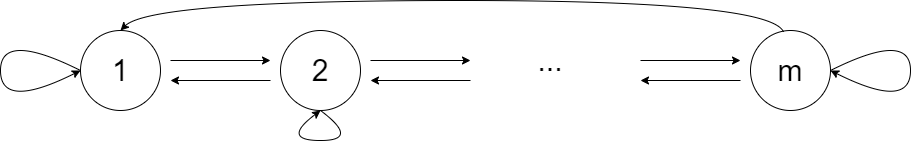
\includegraphics[scale=0.3]{n-state.png}
    \caption{n-state transition diagram}
\end{figure}
\begin{theorem}
    For the m-state Markov chains, and the non-zero terms only have $\{p_{i, i+1}, i=1, \dots m-1\} \bigcup \{p_{i, i-1}, i=2, \dots m-1\} \bigcup \{p_{m,1}\}$, $(w_{c})_{c \in \mathcal{C}_{\infty}}$ satisfies a large deviation principle, and its rate function is
    % \begin{align}
    %     I_{n}^{c'}(\nu) 
    %     % &= \sum_{i, j \in S} \nu_c
    %     % \log \left(\frac{\sum_{c \ni [i,j]} \nu_c}{\nu^i}/ \frac{\sum_{c \ni [i,j]} w_c }{w^i}
    %     % \right) \\
    %     &= \sum_{i\in S} \nu_i \log \left(\frac{\nu_i}{\nu^i} / \frac{w_i}{w^i}\right)
    %     + \sum_{i,j \in S, i<j} \nu_{i,j} \log \left(\frac{\sum_{c \ni [i,j]} \nu_c}{\nu^i}
    %     /\frac{\sum_{c \ni [i,j]} w_c}{w^i}\right)
    %     \left(\frac{\sum_{c \ni (j,i)} \nu_c}{\nu^i}
    %     /\frac{\sum_{c \ni (j,i)} w_c}{w^i}\right) \\
    %     &+ \nu_{12\cdots m} \sum_{i\in S} \log \left(\frac{\sum_{c \ni [i]} \nu_c}{\nu^i}/ \frac{\sum_{c \ni [i]} w_c}{w^i}\right)
    % \end{align}
    \begin{align*}
        I_{m'}^{c}(\nu) = \sum_{i \in S} \sum_{c \ni [i]} \nu_c \log \left(\frac{\nu_c}{\nu^i} /\frac{w_c}{w^i}\right)
    \end{align*}
\end{theorem}
\begin{proof}
    The proof is similar in spirit to that of Theorem 1.1, the main difference lies in the simplification of rate function.
    Let 
    \begin{align*}
        K_n = \biggl\{k=(k_c)_{c\in \mathcal{C}_{\infty}}: \sum_{c \in \mathcal{C}_{\infty}} k_{c} |c| \le n \biggr\},
    \end{align*}
    and
    \begin{align*}
        Q_n(a) = \max_{k\in K_n: \mu_n(k) \in B_a(\nu)} 
        \mathcal{E} (G^{m'} (k)) \Pi_{i,j \in S} p_{ij}^{\sum_{c \ni [i,j]} k_{c}}.
    \end{align*}
    We only need to simply the following formula.
    \begin{align*}
        &\frac{1}{n} \log \mathcal{E} (G^{m'} (k)) \Pi_{i, j \in S} p_{ij}^{\sum_{c \ni [i,j]} k_{c}} \\
        &= -\biggl(
        \sum_{i \in S} \nu_i \log(\frac{1}{p_{i}} \frac{\nu_i}{\nu^i})
        +\nu_{12} \log \frac{1}{p_{12}p_{21}} \frac{\nu_{12}}{\nu_{12}+\nu_{23}+\nu_{12\dots m}} \frac{\nu^1-\nu_1}{\nu^1} \frac{\nu^2 -\nu_2}{\nu^2} \\
        &+\nu_{m-1, m} \log \frac{1}{p_{m-1, m}p_{n,m-1}} \frac{\nu_{m-1, m}}{\nu_{m-1, m}+\nu_{m-2,m-1}+\nu_{12\dots m}} \frac{\nu^{m-1}-\nu_{m-1}}{\nu^{m-1}} \frac{\nu^{m} -\nu_{m}}{\nu^{m}} \\
        &+\sum_{i=2}^{m-2} \nu_{i, i+1} \log (\frac{1}{p_{i, i+1}p_{i+1, i}} 
        \frac{\nu_{i, i+1} (\nu_{i, i+1}+\nu_{1, 2, \dots m})}{(\nu_{i, i+1}+\nu_{i+1, i+2}+\nu_{1, 2, \dots m}) (\nu_{i-1, i}+\nu_{i, i+1}+\nu_{1, 2, \dots m})} 
        \frac{\nu^{i}-\nu_{i}}{\nu^{i}} \frac{\nu^{i+1}-\nu_{i+1}}{\nu^{i+1}})\\
        &+\nu_{1, 2, \dots m} \log (\frac{1}{p_{12}p_{23}\dots p_{m-1, s} p_{s,1}}
        \nu_{1, 2, \dots m} \frac{\Pi_{i=2}^{m-2} (\nu_{i, i+1} + \nu_{1, 2, \dots m})}
        {\Pi_{i=2}^{m-1} (\nu^i - \nu_i)}
        \Pi_{i=1}^{m} \frac{\nu^{i}-\nu_{i}}{\nu^{i}})
        \biggr) \\
        &= -\biggl(
        \sum_{i \in S} \nu_i \log(\frac{1}{p_{i}} \frac{\nu_i}{\nu^i})
        +\nu_{1, 2} \log (\frac{1}{p_{12}p_{21}} \frac{\nu_{12}(\nu^1-\nu_1)}{\nu^1 \nu^2}) 
        +\nu_{m-1, m} \log \frac{1}{p_{m-1, m}p_{n,m-1}} \frac{\nu_{m-1, m}(\nu^{m-1}-\nu_{m-1})}{\nu^{m-1} \nu^{m}} \\
        &+\sum_{i=2}^{m-2} \nu_{i, i+1} \log (\frac{1}{p_{i, i+1}p_{i+1, i}} 
        \frac{\nu_{i, i+1} (\nu_{i, i+1}+\nu_{1, 2, \dots m})}{\nu^{i} \nu^{i+1}} ) \\
        &+\nu_{1, 2, \dots m} \log (\frac{1}{p_{12}p_{23}\dots p_{m-1, m} p_{m,1}}
        \nu_{1, 2, \dots m} \frac{\Pi_{i=1}^{m-1} (\nu_{i, i+1} + \nu_{1, 2, \dots m})}{\Pi_{i=1}^m \nu^{i}}
        \biggr) \\
    \end{align*}
    Because $p_{ij} = \frac{\sum_{c \ni [i,j]} w_c}{\sum_{c \ni (i)} w_c}$, and $w$ substitute for $p_{ij}$ in th formula above, the rate function $I_{n}^{c'}(\nu)$ would be obtained. The rest proof is same as Theorem 1.1.
\end{proof}
\begin{corollary}
    $I_{n'}^{c}(\nu)$ is  finite, continuous, positive and strictly convex
\end{corollary}
\begin{proof}
    The finiteness and continuity is obvious, and we also can employ Log-sum inequality to proof its positivity convexity.
\end{proof}

\section{Appendix}
Consider the first n-step of the above Markov chains $(\xi_l)$, we assume that $\xi_{n}=\xi_1$, and the number of cycle $c$ occurring is $k_{c}$.
If marking each occurence of state pair $(s, t)$ in $\xi_1, \dots, \xi_n$ by drawing an arrow from $s$ to $t$, we can obtain an oriented graph $G^m(k)$. And we employ $\mathcal{E} (G^m(k))$ to denote the number of Euler circuits on $G^m(k)$, by the way, $\mathcal{E}_i (G^m(k))$ denotes the number of Euler circuits which start from states $i$, i.e. $\xi_1 = i$.

\begin{theorem}
    For the graph $G^m(k)$ induced by the Markov chains $(\xi_l)_{l\ge 0}$, if the size of state space is $s$, then we have the following formula:
    \begin{align*}
        \mathcal{E}_1 (G^m(k)) &= 
        \binom{k_{12}+k_{1m}+k^{+}+k^{-}}{k_{12}, k_{1m}, k^{+}, k^{-}} 
        \binom{k_{1}+k_{12}+k_{1m}+k^{+}+k^{-}}{k_{12}+k_{1m}+k^{+}+k^{-}}
        \biggl[\Pi_{i\in S, i\neq 1} \binom{\sum_{c \ni [i]} k_{c} - 1}{\sum_{c \ni [i]} k_{c} - k_{i} - 1}\biggr]\\
        &\biggl[\sum_{k_{23}^{+}+k_{23}^{-}=k_{23}} \sum_{k_{34}^{+}+k_{34}^{-}=k_{34}}
        \dots \sum_{k_{m-1,m}^{+}+k_{m-1,m}^{-}=k_{m-1,m}}
        \binom{k_{23}^{+}+k_{12}+k^{+}-1}{k_{23}^{+}} \binom{k_{34}^{+}+k_{23}^{+}+k^{+}-1}{k_{34}^{+}} \\
        &\dots \binom{k_{m-1, m}^{+}+ k^{+}_{m-2, m-1} + k^{+}  -1}{k_{m-1, m}^{+}} \binom{k_{1, m} + k_{m-1, m}^{-} + k^{-} -1}{k_{m-1, m}^{-}} \binom{k_{m-1, m}^{-} + k_{m-2, m-1}^{-} + k^{-} - 1}{k_{m-2, m-1}^{-}} \\
        &\dots \binom{k_{23}^{-} + k_{34}^{-} + k^{-} - 1}{k_{23}^{-}}\biggr]
    \end{align*}

    where $k^{+}$ and $k^{-}$ are the number of cycle $\{1, 2, \dots, s\}$ , $\{s, m-1, \dots, 1\}$ respectively. And $k_{s, t}^{+}$ represents the number of cycles of which the state $s$ occurring fistly among cycles $\{s, t\}$, so $k_{s, t}^{-}$ is number of remains.
\end{theorem}
\begin{proof}
    We use following three steps to count all the Euler circuits.
    1. This Markov chains starts from state 1, hence we pick the cycles which includes state 1, i.e. $\{1\}$, $\{1, 2\}$, $\{1, m\}$, $\{1, 2, \dots, m\}$, $\{1, \dots, m-1,m, 2\}$. And line them up, the number of permutations is:
    \begin{align*}
        \binom{k_{1}+k_{12}+k_{1m}+k^{+}+k^{-}}{k_{1}, k_{12}, k_{1m}, k^{+}, k^{-}}
    \end{align*}
    
    2. Next we need to insert the other 2-state cycles into it based on above permutation.
    For the cycle $(s-1, s)$, $s \in \{3, 4, \dots , m\}$, it firstly be inserted into the cycle $(1, 2, \dots, m)$ and $(s-2, s-1)$ which start from state $s-2$ if $s \neq 3$.
    The cycle $(s-1, s)$ that has been inserted all states from state $s-1$, next we insert the remains that starts from state $s$, the optional cycles have $(1, s, m-1, \dots, 2)$ and $(s, s+1)$ which start from state $s+1$ if $s \neq m$. ~\ref{fig:insert1} illustrates the way to insert 2-state cycles.\\
    If we change the order of inserting, the cycle would not occurr at the inserting point, such as ~\ref{fig:insert2}
    \begin{align*}
        &\sum_{k_{23}^{+}+k_{23}^{-}=k_{23}} \sum_{k_{34}^{+}+k_{34}^{-}=k_{34}}
        \dots \sum_{k_{m-1,m}^{+}+k_{m-1,m}^{-}=k_{m-1,m}}
        \binom{k_{23}^{+}+k_{12}+k^{+}-1}{k_{23}^{+}} \binom{k_{34}^{+}+k_{23}^{+}+k^{+}-1}{k_{34}^{+}} \\
        &\dots \binom{k_{m-1, m}^{+}+ k^{+}_{m-2, m-1} + k^{+}  -1}{k_{m-1, m}^{+}} \binom{k_{1, m} + k_{m-1, m}^{-} + k^{-} -1}{k_{m-1, m}^{-}} \binom{k_{m-1, m}^{-} + k_{m-2, m-1}^{-} + k^{-} - 1}{k_{m-2, m-1}^{-}} \\
        &\dots \binom{k_{23}^{-} + k_{34}^{-} + k^{-} - 1}{k_{23}^{-}}
    \end{align*}
    \begin{figure}[h] \label{fig:insert1} 
        \centering
        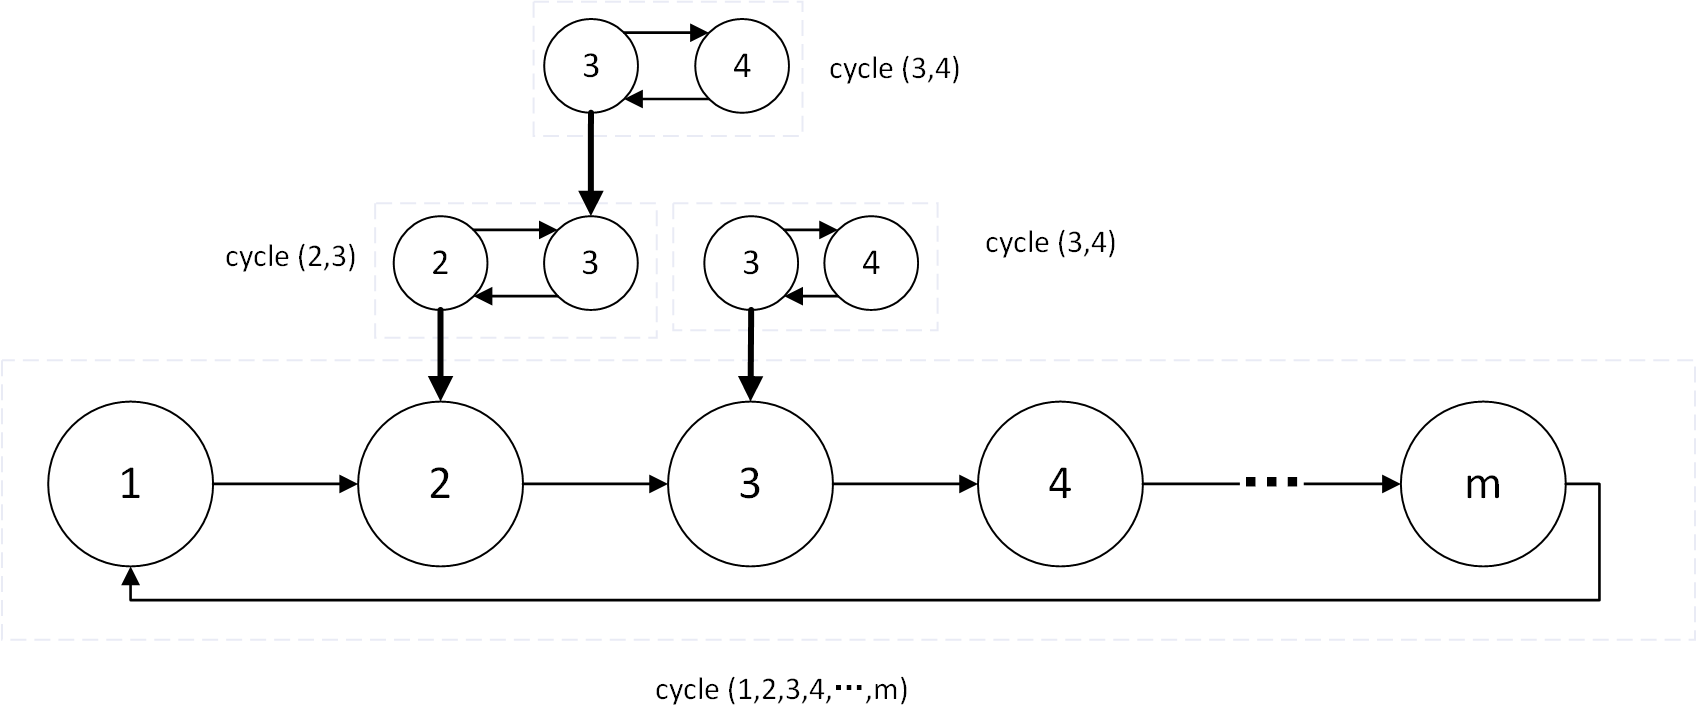
\includegraphics[scale=0.5]{insert1.png}
        \caption{Right Insertion}
    \end{figure}
    \begin{figure}[h] \label{fig:insert2} 
        \centering
        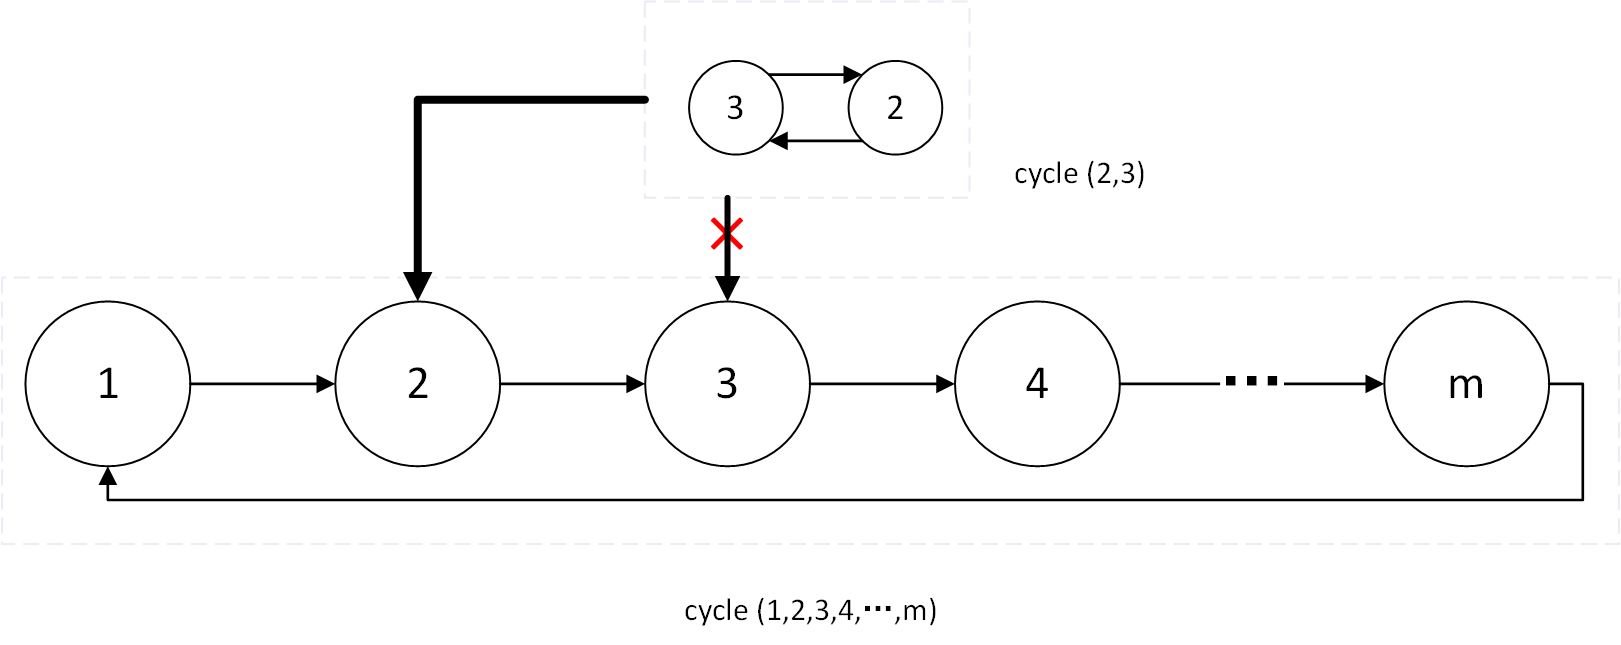
\includegraphics[scale=0.5]{insert2.png}
        \caption{Wrong Insertion}
    \end{figure}

    3. Consider the one of the  above permutation, we insert the other 1-state cycles into it, i.e. $(2)$, $(3)$, \dots, $(s)$.  The number of permutations is:
    \begin{align*}
        \Pi_{i\in S, i\neq 1} \binom{\sum_{c \ni [i]} k_{c} - 1}{\sum_{c \ni [i]} k_{c} - k_{i} - 1}
    \end{align*}
\end{proof}

\begin{corollary}
    If $p_{1m}=0$, the number of Euler circuits is 
    \begin{align} \label{eq:12}
        \mathcal{E} (G^{m'} (k))
        = \exp(O \log n)  \binom{k_{12}+k_{1,2\dots ,m}}{k_{12}} 
        \Pi_{i=2}^{m-1} \binom{k_{1,2\dots ,m}+ k_{i-1, i}+ k_{i, i+1}}{k_{i, i+1}}
        \Pi_{i \in S} \binom{\sum_{i\ni c} k_{c}}{\sum_{i\ni c} k_{c} - k_{i}}
    \end{align}
\end{corollary}
\begin{proof}
    Because $p_{1m}=0$, $k^-=0$, we do not need to consider insert 2-state cycle  into $(1,m)$ and $(1, m, m-1, \dots, 2)$. Compairing to Theorem 2.1, only the second step is different, it is:
    \begin{align*}
        \Pi_{i=2}^{m-1} \binom{k_{1,2\dots ,m}+ k_{i-1, i}+ k_{i, i+1}}{k_{i, i+1}}
    \end{align*}
    In addition, the path starting from other states which is not state 1 should be considered, so
    \begin{align*}
        \mathcal{E} (G^{m'} (k))
        &\le  n \binom{k_{12}+k_{1,2\dots ,m}}{k_{12}} 
        \Pi_{i=2}^{m-1} \binom{k_{1,2\dots ,m}+ k_{i-1, i}+ k_{i, i+1}}{k_{i, i+1}}
        \Pi_{i \in S} \binom{\sum_{i\ni c} k_{c}}{\sum_{i\ni c} k_{c} - k_{i}}\\
    \end{align*}
    We can get ~\ref{eq:12}.
\end{proof}

\begin{corollary}
    Consider the graph $G(k)$ induced by the Markov chains $(\xi_l)_{l\ge 0}$.
    If $s= 2$, we have:
    \begin{align*}
        \mathcal{E} (G^2(k))= \exp(O \log n) \binom{k_{1} + k_{12}}{k_{1}} \binom{k_{2}+k_{12}}{k_{2}}
    \end{align*}
    
    If $s= 3$, we have:
    \begin{align*}
        \mathcal{E} (G^3(k))= 
        &\exp(O (\log(n))) \binom{k_{12} + k_{13} + k_{123} +k_{132}}{k_{12}, ~k_{13}, ~k_{123}, ~k_{132}} \\
        & \binom{k_1 + k_{12} + k_{13} + k_{123} +k_{132}}{k_1}
        \binom{k_{12} +k_{13} + k_{123} +k_{132} + k_{23}}{k_{23}} \\
        &\binom{k_{12} + k_{123} + k_{132} +k_{23} +k_2}{k_2} \binom{k_{13} +k_{123} +k_{132} +k_{23} +k_3}{k_3}
    \end{align*}
\end{corollary}

\
\end{document}